\documentclass[twoside,onecolumn,11pt]{article}
% \documentclass[twocolumn, prX]{revtex4}

\usepackage[margin=1in]{geometry}
\usepackage{amsmath,amssymb,mathabx,enumitem,graphicx,subfigure,authblk}
% \usepackage{xcolor} \pagecolor[rgb]{0.2,0.2,0.2} \color[rgb]{1,1,1}
\usepackage{xcolor}
\usepackage{enumitem}
\setlist[itemize]{noitemsep} % Make itemize lists more compact

\usepackage{abstract} % Allows abstract customization
\renewcommand{\abstractnamefont}{\normalfont\bfseries} % Set the "Abstract" text to bold
\renewcommand{\abstracttextfont}{\normalfont\small\itshape} % Set the abstract itself to small italic text

\usepackage{biblatex}
\addbibresource{reference.bib}

\usepackage{titlesec} % Allows customization of titles
\renewcommand\thesection{\Roman{section}} % Roman numerals for the sections
% \renewcommand\thesubsection{\roman{subsection}} % roman numerals for subsections
\titleformat{\section}[block]{\large\scshape\centering}{\thesection.}{1em}{} % Change the look of the section titles
\titleformat{\subsection}[block]{\large}{\thesubsection.}{1em}{} % Change the look of the section titles

\usepackage{lettrine}

\usepackage{titling} % Customizing the title section

% Calculus
\newcommand{\dx}{\mathrm d}
\newcommand{\ddx}[2]{\frac{\mathrm d #1}{\mathrm d #2}}
\newcommand{\pdx}[2]{\frac{\partial  #1}{\partial  #2}}
\newcommand{\fdx}[2]{\frac{\delta  #1}{\delta  #2}}
\newcommand{\intfty}{\int_{-\infty}^{\infty}}

% Quantum
\newcommand{\bra}[1]{\left\langle #1 \right\rvert}
\newcommand{\ket}[1]{\left\lvert #1 \right\rangle}
\newcommand{\expv}[1]{\left\langle #1 \right\rangle}
\newcommand{\braket}[2]{\left\langle #1 \!\left\vert\vphantom{#1#2}\right.\! #2 \right\rangle}
\newcommand{\fslash}[1]{\setbox 0 \hbox{$#1$} \rlap{\hbox to \wd 0 {\hss/\hss}} \box 0}

% Misc
\newcommand{\abs}[1]{\left\lvert #1 \right\rvert}
\newcommand{\rfrac}[2]{\frac{#2}{#1}}
\newcommand{\pfrac}[2]{\left(\frac{#1}{#2}\right)}
\newenvironment{itemalign}{\hfil $ \displaystyle \begin{aligned}[t]}{\end{aligned} $}
\DeclareMathOperator{\erfc}{erfc}
\newcommand*{\rom}[1]{\expandafter\@slowromancap\romannumeral #1@}
\newcommand{\RNum}[1]{\uppercase\expandafter{\romannumeral #1\relax}}

\newcommand{\aaa}{a}

\title{How generic is eternal inflation?}% \\ \vspace{.3cm} \Large{[Working Title]}}
\author{Ross N. Greenwood${}^\dag$, Anthony Aguirre${}^\dag$}
\affil{$^\dag$University of California, Santa Cruz}
\renewcommand{\maketitlehookd}{%
\begin{abstract}
It is widely believed that an eternal multiverse is a generic prediction of cosmic inflation, arising without the need for fine-tuning of the model parameters or initial conditions.  However, that belief rests on largely anecdotal evidence based on a small number of familiar inflation models -- not the conclusions of a direct, comprehensive analysis.  In this work, we set out to quantify the degree to which eternal inflation is a generic feature of single-field models, laboring under only the most basic assumptions regarding the initial state of the inflaton field and the potential function governing its dynamics.

\end{abstract}
}

\begin{document}

%  	\maketitle
%  	\tableofcontents
 	
    
A straight-forward reading of what has become the standard model of cosmology comes with it a strong implication that our observable universe may be just one patch of an infinite and growing multiverse
, in which the runaway expansion that shaped our deep past continues forever throughout much of space.  It is widely believed that this eternal multiverse is a generic prediction of cosmic inflation -- a free side effect arising without the need for fine-tuning of model parameters or initial conditions.  As inflation continues to gather empirical support as an explanatory account of our cosmic history, it remains an open question whether eternal inflation is truly generic among candidate models consistent with observation.

In this work, we set out to quantify the degree to which eternal inflation is a generic feature of single-field inflation models.  In other words: what is the likelihood of finding ourselves in an eternally inflating multiverse?  In addressing this question, we labor under only the most basic assumptions regarding the initial state of the inflaton and the potential function governing its dynamics.  Where quantitative analysis is no longer feasible, we attempt to paint a qualitative picture informed by mathematical considerations, and suggest steps toward developing clarity.

\paragraph{Overview}

In Section \RNum 1, we review the physics of eternal inflation and the criteria for its three distinct modes: false-vacuum, stochastic, and topological.  We discuss the implications of eternal inflation for cosmology, and take account of the established wisdom regarding the question of its prevalance among possibly predictive models of inflation.

In Section \RNum 2, we define the critera for eternal inflation to be considered {generic} (or equivalently: {\it prevalent}, {\it typical}) within the space of single-field inflation scenarios that lie within the scope of this analysis.  
We discuss the inherent non-uniqueness of the probability measure over inflaton potential functions and initial conditions, and identify some properties of the measure that we expect to enhance the statistical weight of conclusions to be drawn from it.

In Section \RNum 3, we address the prevalence of eternal inflation analytically.  
We review and expand upon several no-go theorems published in recent years, which set out criteria under which inflation is not generically eternal.  
To explore the application of these analytical constraints, we perform an in-depth analysis of hybrid inflation -- a model for which inflation is known to be non-eternal given most choices of parameters and initial conditions that are consistent with observation.

In Section \RNum 4, we take account of the gaps left in our understanding after having exhausted analytical resources, and employ numerical methods to further assess the typicality of eternal inflation.  
We simulate the dynamics of inflation across an ensemble of randomly generated potential functions and initial conditions, experimenting with several candidate measures.

In Section \RNum 5, we discuss conclusions to be drawn from this study, and suggest avenues for future work.

    \section{Background and Motivation}

\subsection{Three Roads to Eternal Inflation}

% In order that matter and galaxies could to have come to populate our observable universe, inflation must have come to an end within our Hubble volume.  The timing of that transition may in general vary across large distance scales with the local behavior of the inflaton fields, leading to the partition of space into non-inflating {\it pocket universes} embedded in an inflating background.  If the inflating volume consistently reproduces faster than these pocket universes can form, then the cycle will continue without indefinitely.  This scenario is known as {\it eternal inflation}.

Eternal inflation may manifest in any of three discernable modes: stochastic, topological, and false-vacuum.  More than one mode may manifest in a given inflation model, but only one of the associated criteria need be be satisfied to all but ensure ever-lasting inflation.  As such, those wishing to mount a defense against the creeping inevitability of eternal inflation must be guarded on three sides.

\textbf{Stochastic eternal inflation} occurs when quantum fluctuations of the inflaton field dominate over its classical evolution according to the slow roll equation of motion.
Over the passage of a Hubble time $H^{-1}$, the field expectation value $\phi$ decreases by an amount $\Delta \phi = \lvert\dot\phi\rvert H^{-1} = V_{,\phi} / 3H^2 $ as it classically rolls.  During the same interval, quantum fluctuations with amplitude $\delta\phi \approx H/2\pi$ may drive the field up or down the potential slope relative to its classical trajectory.  
If in that time, the probability for the field within an initially Hubble-sized region to move up the slope is greater than the ratio of initial to final volumes ($1/e^3$), then at least one final Hubble volume is likely to continue inflating after a time $H^{-1}$.  This occurs when $ \Delta \phi \lesssim \delta \phi \, \sqrt{2} \, \erfc^{-1} (2e^{-3}) $ or
\begin{equation}
% \delta\phi \gtrsim 0.61 \, \Delta\phi 
V^{3/2} \geq 6.64 \, V_{,\phi} \label{seic}
\end{equation}  
We refer to this as the {\it stochastic eternal inflation criterion}.

\textbf{Topological eternal inflation} may manifest in cases when spatially inhomogeneous field solutions are divisible into (approximately) inequivalent homotopy classes.  
Consider for example a symmetric potential with two degenerate vacua at $\phi = \pm \phi_0$, separated by a local maximum at $\phi = 0$.  
If in neighboring regions the field has settled into different vacua, then by continuity the field must reach the maximum of the potential somewhere in between.  
This configuration cannot classically evolve into a true vacuum solution, as that would require the energy to increase as the field in one region traverses the central maximum.
If the space occupying the middle ground is undergoing inflationary expansion at a rate sufficient to compensate for the recession of its boundaries, then we have {topological eternal inflation}.

In \textbf{false-vacuum eternal inflation}, the field becomes trapped near a local minimum of the potential, corresponding to a positive vacuum energy.  Classically, the field would be stuck there indefinitely.  However, quantum effects allow it to ``escape'' by tunneling out of this false vacuum to continue its descent toward an even lower minimum.
If the tunneling rate is sufficiently small, then the volume of space that exits inflation in this manner is replaced by the expansion of neighboring regions that do not.  The volume of inflating space never decreases, even as its fraction of the total volume may tend toward zero.



\subsection{Implications for Cosmology}



\subsection{But is it generic?} 

Eternal inflation is assumed by many in the field to be a generic feature of inflation \cite{guth07}.  What is the basis for this assumption, and how did it come to be accepted?  Does the common standard for generic agree with the one adopted in this paper?  Why or why not?  Why is the justification for the prevailing view insufficient, and what more is left to be desired?  How do we claim our results go further in addressing this question?

Check which models are compared with experimental results in the Planck and WMAP papers.

In \cite{mersiniparker07}, it is argued that application of an adiabatic regularization procedure in the calculation of the amplitude of quantum fluctuations is responsible for increasing the energy cost of stochastic eternal inflation to prohibitively high levels.



    \section{Desperate Measures}

In order to make sensible statistical statements about the prevalence of eternal inflation, we must identify the set $\Omega$ of possible outcomes under consideration, and then establish a system for assigning probabilities to those various outcomes.  
In our context, we take $\Omega$ to be the set of viable inflation scenarios -- pairings of a potential function and initial conditions.  

The probability {\it measure} is a map $\mu : 2^\Omega \to \mathbb R$ from possible sets of draws from the ``hat'' $\Omega$ to the interval $[0,1]$.  The measure assigns a probability to each set of outcomes, such that $\mu(\bigwedge_i x_i) = \sum_i \mu(x_i)$ for disjoint sets $x_i \in 2^\Omega$,
% $\mu(x) \leq \mu(x \bigcup y) \,\forall\, x,y \in 2^\Omega$, 
with $\mu(\emptyset)=0$ and $\mu(\Omega) = 1$.
Unlike the measures on the volume of Euclidean space ($\dx x \wedge \dx y \wedge \dx z$) or on rolls of a weighted die, the measure in our case is ambiguous; there is no physically preferred way of assigning probabilities to the space of inflation scenarios.

Can we find a measure in which eternal inflation is not generic, which is reasonably simple and not cheating?

What about the No-Boundary Measure or a measure that exponentially favors low energies.

It is likely not reasonable to expect that the measures on the potential $V(\phi)$ and the initial conditions $\mathbf p$ are separable, such that their joint measure would take the form $\mu(V,\mathbf p) = \mu(V) \mu(\mathbf p)$.  (A counterexample might be found within the subspace consisting of quadratic potentials, in which arbitrarily large field values may be disfavored on physical grounds.)





\subsection{Measures on Potentials}

If the inflaton is to be treated as a fundamental quantum field, then the classical potential to which the expectation value of the inflaton is approximately subject will the expectation value of an operator-valued function of the field operator: $V(\phi) \approx \bra{\Psi} V(\hat \phi) \ket{\Psi}$.  If the field is allowed to take values comparable to the Planck mass, then we may construct a potential with any number of terms containing even or odd powers of the field operator, so long as the potential is bounded from below.  
% If such a potential possesses broken symmetry, then expanding the potential around the nonzero vacuum expectation value will likely yield terms that are odd powers of the field operator.  
If the field is coupled to additional fields with vacuum expectation values and that vary slowly in time, then such interaction terms would be even-powered.


While the potential function may contain odd terms in the series expansion, it must be bounded from below.  Even if we restrict the function space of potentials to the square integrable functions $L^2$.


\begin{itemize}
    
    \item Weigh potentials by their complexity -- by the number of interactions with unmodeled free fields that would be necessary to produce the potential.
    \item Weigh potentials by their degree of departure from plausible potentials for elementary fields in quantum field theory.

\end{itemize}

If we assume that the inflaton is a quantum scalar field expanded about some minimum in its potential, what assumptions can we then make about the form of that potential?

\paragraph{Reconstructing the Potential}

\subsection{Measures on Initial Conditions}

    The initial conditions in our models are the values of the homogeneous scalar field $\phi$ and its time derivative.  A simple example of a measure over initial field values is $\mu(\Delta) = \int_\Delta \dx \phi$, where $\Delta$ is some finite (or infinitesimal) interval in field space.  This measure assigns equal probability to all field values.
    
    Tegmark \cite{tegmark08} adopted two measures on the space of initial conditions:
    \begin{description}
    
        \item[Measure A] {\it Assign equal marginal probability to the field values that maximize the potential function, and zero probability to all other field values.} %, unit marginal probability to $\dot\phi = 0$.
        
        In this case, we are sampling half-basins of the potential, accounting for any inflation that occurs between a randomly selected local maximum and a neighboring minimum.  We allow the field to approach the local maximum as $\tau \to -\infty$.
        
        \begin{description}
        \item[Pros] $\dot\phi_0$ given by slow roll equation of motion.
        \item[Cons] There may be inflation higher on the potential, or the inflation epoch into which the field is dropped may have already generated enough e-folds of expansion to satisfy the bound on $N$.
        \end{description}
        
        \item[Measure B] {\it Assign equal marginal probability to all field values.  Discard scenarios in which slow roll conditions are not met at $\phi_0$. % unit marginal probability to $\dot\phi = 0$.
        }
        
        This is equivalent to dropping the field at a random point and starting the clock wherever it lands.  Since in the end we intend to condition our probabilities on the presence of inflation, we lose nothing by discarding scenarios in which the initial field value does not fall within an inflating region of the potential.
        
        \begin{description}
        \item[Pros] $\dot\phi_0$ given by slow roll equation of motion.
        \item[Cons] There may be inflation higher on the potential, or the inflation epoch into which the field is dropped may have already generated enough e-folds of expansion to satisfy the bound on $N$.
        \end{description}
        
    \end{description}
    
    These measures were chosen in part because they allow us to set $\dot\phi$ to zero while maintaining some peace of mind.
    
    Adopting Measure B would lead to a unit probability of encourering stochastic eternal inflation, since the criterion \eqref{seic} is always satisfied when $V_{,\phi} \to 0$.


    \section{Analytical Inroads}

Under what circumstances can we rule out eternal inflation within a family of models by appeal to mathematical criteria?

\subsection{Negative Running}

In \cite{kinneyfreese15}, it was shown that a sufficiently negative value of the running of the spectral index corresponds to failure of the stochastic eternal inflation criterion \eqref{seic}.

The scalar spectral index is defined to be $ n_s(k) \equiv \left. \dx({\ln P_s})/\dx({\ln k}) \right\rvert_{k=k_\star}$, 
% evaluated at some pivot scale $k_\star$,
where $P_s(k)$ is the power spectrum for scalar curvature perturbations.
The running of the spectral index is then defined
$ \alpha \equiv \dx{n_s}/\dx({\ln k}) $.
The stochastic eternal inflation criterion may be expressed in terms of the amplitude of curvature perturbations for modes crossing the Hubble horizon:
\begin{equation} 1 \lesssim \frac{\delta\phi}{\Delta\phi} = \frac{H^2}{2\pi \dot\phi} = \left. \vphantom{\sum} P(k) \right\rvert_{H/2\pi} \label{neg_running} \end{equation}
If we assume that the running of the spectral index is a constant, we may use this relation to compute a lower bound on the running for which this criterion is satisfied.  Plugging in estimates for observables based on measured data, Kinney and Freese found that this bound is negative and quite small in magnitude.

The negation of constraint \eqref{neg_running} expressed in terms of $\ln P$ may be written as follows:
% \[ P(k) = P_\star \left( \frac{k}{k_\star} \right)^{ n_s -1 + \alpha \ln (k/k_\star) + \cdots} < 1 \]
\[ \ln P(k) = \ln P_\star + \left[ n_s -1 + \alpha \ln \frac{k}{k_\star} + \cdots \right] \ln \frac{k}{k_\star} < 0 \]
where $P_\star$ and $k_\star$ are evaluated at some pivot scale.  Plugging in the value $k_\text{max}$ that maximizes $\ln P$:
% \[ \ddx{\ln P(k)}{\ln k} = n_s -1 + 2 \alpha \ln \frac{k}{k_\star} < 0 \] 
% \[ \ln \frac{k_\text{max}}{k_\star} = \frac{1 - n_s}{2\alpha} \]
% \[ \ln P(k_\text{max}) = \ln P_\star + \frac{(n_s-1)(1-n_s)}{2\alpha} + \frac{\alpha(1-n_s)^2}{4\alpha^2} \]
\[ \ln P(k_\text{max}) = \ln P_\star - \frac{(1-n_s)^2}{4\alpha} < 0 \]
Accepting this as our ultimate upper bound on $\ln P$, we obtain an upper bound on the running $\alpha$
\[ \alpha < \frac{(1-n_s)^2}{4\ln P_\star} < -4 \times 10^{-5}, \]
where we have plugged in the measured values of the power spectrum at the pivot scale $P_\star \approx 2 \times 10^{-9}$ and the scalar spectral index $1 - n_s < 0.06$.
% \[ \alpha < -4 \times 10^{-5} \]

% Manipulating the expression for the number of e-foldings of slow-roll inflation $N \equiv \ln k$ in terms of the potential $V(\phi)$, we obtain (pivot scale suppressed)
% \[ \dx \!\left(\ln k \right) = - (V_{,\phi}/V) \dx\phi = - \dx \!\left(\ln V\right) \]
% Using this relation, we may express the spectral index and running in terms of the potential $V(\phi)$.

\subsection{Non-Eternal Hybrid Inflation}

While eternal inflation is thought to be generic, there are families of models within which inflation is not typically eternal.  We begin by performing an in-depth analysis of eternal inflation in hybrid models.




% \paragraph{The Model}

The model of {\it hybrid inflation} proposed by Linde \cite{linde1994hybrid} 
% that produced inflation with coupling parameters of order one, eliminating the need for fine-tuning.  
posits two coupled scalar fields -- the inflaton $\phi$ and a Higgs-like {\it timer} field $\sigma$ -- governed by the potential
\begin{equation} V(\phi,\sigma) = \frac12{m^2} \phi^2 + \frac1{4\lambda} (M^2 - \lambda \sigma^2)^2 + \frac12{g^2} \phi^2 \sigma^2. \label{pot} \end{equation}
Here the parameters $m$ and $M \gg m$ have dimensions of mass, while $g$ and $\lambda$ are dimensionless.  

% \begin{figure}[h]
%     \centering
%     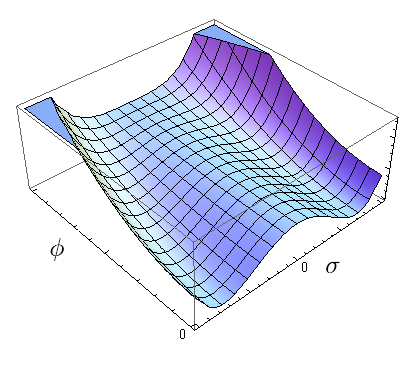
\includegraphics[width=7cm]{Figures/hybridpotential}
%     \caption{The potential $V(\phi,\sigma)$ of hybrid inflation.}
% \end{figure}

The curvature of the potential with respect to $\sigma$ is given by $M_\sigma^2(\phi) \equiv g^2\phi^2 - M^2$; so if $\phi$ starts out much larger than the critical value $\phi_c \equiv M/g$, then the curvature in $\sigma$ is positive and correspondingly large.  In such cases, the system quickly settles to the local minimum at $\sigma = 0$, marking the floor of the super-critical {\it inflationary valley}.  
% In this regime, the hybrid model behaves effectively as a single-field quadratic model, resembling old inflation with an additional vacuum term.  
The potential \eqref{pot} is then
\begin{equation} V(\phi,0) = \frac12 m^2 \phi^2 + \frac{M^4}{4\lambda} = \frac12 m^2 \left( \phi^2 + \aaa^2 \right), \label{valley} \end{equation}
where $\aaa^2 \equiv M^4/2\lambda m^2$ .
% and $M_P \equiv (8\pi G)^{-1/2}$ is the reduced Planck mass.  
(Here we work in Planck units where $M_P \equiv (8\pi G)^{-1/2} = 1$.)
% (Here we introduce an overline notation, indicating that the overlined quantity 
% is expressed in natural units, with $M_P = 1$:
% has been made dimensionless by adding or removing powers of $M_P$: 
% $m \equiv m/M_P$, $\phi \equiv \phi/M_P$, $\widebar V \equiv V/M_P^4$, etc.)
The slow roll evolution of the initially large $\phi$ field is interrupted by a symmetry-breaking phase transition at $\phi = \phi_c$, after which the curvature in $\sigma$ becomes negative.  
The system then rapidly rolls down to one of the two global minima at $\phi=0,\;\sigma=\pm M/\sqrt{\lambda}$.  If $ M^3 \ll \sqrt{\lambda} g m$, then inflation ends within one $e$-folding of expansion after reaching $\phi_c$.
The following parameter values offered in \cite{linde1994hybrid} result predictions that agree with observed features of the scalar density perturbation spectrum: 
% \[ M \sim 10^{11} \text{ GeV} \qquad m \sim 10^2 \text{ GeV} \qquad g^2 \sim \lambda \sim 0.1 \]
\[ M \sim 10^{-8} M_P, \quad m \sim 10^{-17} M_P, \quad g^2 \sim \lambda \sim 0.1 \]

% The regimes are denoted by the relation of $\phi$ to the dimensionless parameter $a \equiv M^4/2\lambda m^2$.  For $\phi \gg a$, the potential is mass dominated; for $\phi \ll a$, it is vacuum dominated.

% \subsubsection{Density Perturbations}

% \begin{enumerate}[label=\arabic{*}.]
% \item $ Q_s = \dfrac{V^{3/2}}{\pi \sqrt{75} \, M_P^3 \, m^2 \phi } = (1.945 \pm 0.052) \times 10^{-5} $
% \item $ n_s - 1 = \dfrac{2 m^2}{V} \left( 1 - \dfrac{3 \, m^2 \phi^2}{2 V} \right) M_P^2 = -0.047 \pm 0.016 $
% \item $ \alpha_s = \dfrac{4 m^4 \phi^2}{V^2} \left( \dfrac{2 m^2}{V} - \dfrac{ 3 m^4 \phi^2}{2 V^2} \right) M_P^4 = -0.040 \pm 0.027 $
% \end{enumerate}

% \paragraph{Number of e-foldings}

Let us assume that inflation ends so abruptly when $\phi$ reaches the critical value $\phi_c$ from above.  The number of $e$-foldings of inflation, $N$, elapsed between the imprinting of CMB density perturbations and the end of inflation must be between 50 and 60, with 55 being an acceptable figure for our purposes.  
% We will find it useful to parameterize the trajectory of the homogeneous $\phi$ field in terms of the number of e-foldings remaining until the end of inflation.
% Reversing the integral expression for $N$ yields a differential equation for $\phi(N)$:
% \[ \ddx{\phi}{N} = \frac{ 2 \phi }{ \phi^2 + \aaa^2 } \]
The initial value $\phi_0$ from which the descent to $\phi_c$ produces $N$ $e$-folds of inflation is then
\begin{equation} \phi_0^2(N) = \aaa^2 \, W \left[ \frac{\phi_c^2}{\aaa^2} \exp \left(\frac{ 4 N + \phi_c^2 }{\aaa^2} \right) \right], \end{equation}
where $W(z)$ is the product logarithm (defined such that $\phi_0(0) = \phi_c$).  
For $\phi_c < M_P$, there exists a threshold near $N \sim \aaa^2$ at which $\phi_0(N)$ changes from $\ll M_P$ to $> M_P$, as shown in Figure \ref{phi_vs_N_a}.  




Since the potential $V(\phi,\sigma)$ exhibits no false vacua, we are left with the possibilities of stochastic and topological eternal inflation. 

\subsubsection{Stochastic Eternal Inflation}

% If eternal inflation is found to occur for field values not far outside the range from which density perturbations are likely to have been imprinted, then it would be difficult to argue that eternal inflation is generically absent from the model.

When restricted to the inflationary valley, the stochastic eternal inflation criterion \eqref{seic} becomes 
\begin{equation} m^2 \phi \lesssim 0.15 \, V^{3/2}. \label{hybrid_seic} \end{equation}
% where $M_P = (8\pi G)^{-1/2}$ is the reduced Planck mass.
where $V = V(\phi,0)$ takes the form \eqref{valley}.

% It is useful to identify two regimes of approximation, in which the potential is dominated by either the quadratic term, $\frac12 m^2\phi^2$ ($\phi \gg \aaa$), or the vacuum term, $M^4/4\lambda$ ($\phi \ll \aaa$).
% \begin{enumerate}
% \item the quadratic term, $\frac12 m^2\phi^2$ ($\phi \gg a$), or
% \item the vacuum term, $\frac1{4\lambda} M^4$ ($\phi \ll a$).
% \end{enumerate}

% By combining the following conditions, we find the constraints under which eternal inflation is allowed.
% \begin{enumerate}
% \item Slow roll conditions
%     \begin{enumerate}[label=\arabic{*}.]
%     \item $\epsilon_\phi = \dfrac{m^4\phi^2}{2V^2} \ll M_P^{-2}$
%     \item $\eta_\phi = \dfrac{m^2}{V} \ll M_P^{-2}$
%     \end{enumerate}
% \item Criterion for eternal inflation: $\phi \lesssim \dfrac{\widebar V^{3/2}}{m^2} \dfrac{M_P}{6.64} $
% \item Observed spectrum of density perturbations
%     \begin{enumerate}[label=\arabic{*}.]
%     \item 
% $ Q_s = \dfrac{V^{3/2}}{\pi \sqrt{75} \, M_P^3 \, m^2 \phi } = (1.945 \pm 0.052) \times 10^{-5} $
%     \item $ n_s - 1 = \dfrac{2 m^2}{V} \left( 1 - \dfrac{3 \, m^2 \phi^2}{2 V} \right) M_P^2 = -0.047 \pm 0.016 $
%     \item $ \alpha_s = \dfrac{4 m^4 \phi^2}{V^2} \left( \dfrac{2 m^2}{V} - \dfrac{ 3 m^4 \phi^2}{2 V^2} \right) M_P^4 = -0.040 \pm 0.027 $
%     \end{enumerate}
% \end{enumerate}
% $ \alpha_s = \dfrac{4 m^4 \phi^2}{V^2} \left( \dfrac{2 m^2}{V} - \dfrac{ 3 m^4 \phi^2}{2 V^2} \right) M_P^4 = -0.040 \pm 0.027 $
% \paragraph{Quadratic Approximation}%: $V(\phi,0) \approx \dfrac12 m^2 \phi^2$}

In the \textbf{quadratic approximation} $\phi \gg \aaa$, the inflaton behaves like a free field with mass $m$.  The slow roll conditions are satisfied when $\phi \gg 1$, and the criterion for eternal inflation is \[ \phi \gtrsim 4.3 \, m^{-1/2}.\] %Q_s \gtrsim 0.24 \]
In the regime $\phi_c \lesssim 1$, the value of $\phi$ at 55 e-foldings before the end of inflation asymptotes to approximately $14.83 \, M_P$ as $\aaa \to 0$.  Values of $\aaa$ larger than $\mathcal O(1)$ are excluded by measurements of the spectral index $n_s$.
For $m \ll 1$ and $\phi_c \lesssim 1$, the field cannot satisfy the eternal inflation criterion within $10^{10}$ $e$-folds.
The parameters of the perturbation spectrum for $\phi \approx 14.8 \, M_P$ are given in Table \ref{quadtable}.
% { \def\arraystretch{2.1}
% \begin{table}[h]
% \centering
% % \begin{tabular}{ccll}
% %                 & Expression & $\phi \approx 14.8$ & Measured Value \\
% %     $Q_s$       & $\dfrac{m \phi^2} {2\pi\sqrt{150}}$  &  $\phantom{-}2.8 \, m$  &  $(1.945 \pm 0.052) \times 10^{-5}$
% % \\  $n_s - 1$   & $-8\,\phi^{-2}$               & $-0.036$         & $-0.047 \pm 0.016$
% % \\  $\alpha_s$  & $-32\,\phi^{-4}$              & $-0.00067$       & $-0.040 \pm 0.027$
% % \\  $r$         & $\phantom-64\,\phi^{-2}$      & $\phantom-0.29$  & $\phantom-0.2^{+0.07}_{-0.05}$
% % \end{tabular} 
% \begin{tabular}{ccll}
%                 & $\phi \approx 14.8$ & Measured Value \\
%     $Q_s$       &  $\phantom{-}2.8 \, m$  &  $(1.945 \pm 0.052) \times 10^{-5}$
% \\  $n_s - 1$   & $-0.036$         & $-0.047 \pm 0.016$
% \\  $\alpha_s$  & $-0.00067$       & $-0.040 \pm 0.027$
% \\  $r$         & $\phantom-0.29$  & $\phantom-0.2^{+0.07}_{-0.05}$
% \end{tabular} 
% \caption{Parameters of the density perturbation spectrum in the quadratic approximation.}
% \label{quadtable}
% \end{table} }

% \[ Q_s \approx \dfrac{ m \phi^2} {2\pi\sqrt{150} M_P^3} \approx 2.8 m \approx (1.945 \pm 0.052) \times 10^{-5} \]
% \[ n_s - 1 \approx -\dfrac{8 M_P^2}{\phi^2} \approx -0.047 \pm 0.016 \implies \phi_e \approx 13 M_P \]
% \[ \alpha_s \approx -\dfrac{32 M_P^4}{\phi^4} \approx -0.040 \pm 0.027 \implies \phi_e \approx 5 M_P \]
% \[ r = \frac{2^6 M_P^2}{\phi^2} \overset?< 0.30 \impliedby \phi > 15 M_P \]

% \paragraph{Vacuum Approximation}%: $V(\phi,0) \approx \dfrac{M^4}{4\lambda}$ }

In the \textbf{vacuum approximation} $\phi \ll \aaa$, the first and second slow roll conditions are, respectively, $\phi \ll \aaa^2$ and $\aaa^2 \gg 1$; both are easily met.  
The criterion \eqref{hybrid_seic} is then 
\begin{equation} \phi \lesssim 0.053 \, m \, \aaa^3. \label{hybrid_vacuum_seic} \end{equation}
Given $m \ll 1$ and $\aaa \gg 1$, this too is easily satisfied, meaning that eternal inflation occurs for small field inflation in the vacuum dominated regime with $\sigma = 0$.
For $\phi > \phi_c$, \eqref{hybrid_vacuum_seic} implies a lower bound on the scalar density perturbation amplitude,
% \[ a \gg \phi_c \qquad a^2 \gg \phi_c \qquad a^3 \gtrsim \dfrac{\phi_c}{m} \]
$ Q_s \gtrsim 0.25 $, %4 \times 10^{-3} $
that is larger than the measured value by four orders of magnitude.
Hence density perturbations must have been imprinted at $\phi < \phi_c$.  Not accounting for the effects of departure of $\sigma$ from $0$, the amplitude would match observations for $\phi \approx 2.2 \times 10^{-5} \, \phi_c$.

In the regime $\aaa \gg 1$, 55 e-foldings affects almost no change in the field, and we can approximate $\phi_0 \approx \phi_c$.  
The parameters of the perturbation spectrum are given in Table \ref{vactable}.

% { \def\arraystretch{2.5}
% \begin{table}[h]
% \centering
% \begin{tabular}{ccll}
%                 & $\phi \approx \phi_c$ & Measured Value \\
%     $Q_s$       & $\dfrac{1} {2\pi\sqrt{150}} \dfrac{m \, \aaa^3}{\phi_c}$  &  $(1.945 \pm 0.052) \times 10^{-5}$ \\
%     $n_s - 1$   & $\dfrac{1}{\aaa} \left( 1 - \dfrac{12 \phi_c^2}{\aaa} \right)$  &  $-0.047 \pm 0.016$ \\
%     $\alpha_s$  & $\dfrac{2^{4} \phi_c^2}{\aaa^6} \left(1 - \dfrac32 \dfrac{\phi_c^2}{\aaa^2} \right) $                   & $-0.040 \pm 0.027$ \\
%     $r$         & $\dfrac{32 \, \phi_c^2}{\aaa^2}$  & $\phantom-0.2^{+0.07}_{-0.05}$
% \end{tabular} 
% \caption{Parameters of the density perturbation spectrum in the vacuum approximation.}
% \label{vactable}
% \end{table} }

The slow roll conditions for $\sigma$ in the vacuum approximation are
\[ \lambda \widebar\sigma \abs{\eta^2 - \widebar\sigma^2} \ll m^2 \aaa^2 \quad\text{and}\quad \lambda \abs{\eta^2 - 3\widebar\sigma^2} \ll m^2 \aaa^2,\]
where $\eta \equiv M/\sqrt{\lambda}$.
\[ Q_s \approx \dfrac{g} {8\pi\sqrt{75} \, \lambda^{3/2}} \dfrac{ M^5 }{ m^2 } \approx (1.945 \pm 0.052) \times 10^{-5} \]
% \[ n_s - 1 \approx \dfrac{2\lambda m^2}{M^4} \left( 1 - \dfrac{24 \lambda m^2}{g^2 M^2} \right) \approx -0.047 \pm 0.016 \]
% \[ \alpha_s \approx \dfrac{2^{10} \lambda^3}{g^2} \dfrac{m^6}{M^{10}} \left(1 - \dfrac{3 \lambda }{2 g^2} \dfrac{m^2}{M^2} \right) \approx -0.040 \pm 0.027 \]
% \[ r = \frac{2^8 \lambda^2 M_P^2 \, m^4 \phi^2}{M^8} \overset?< 0.30 \impliedby \phi < \frac{M^4}{m^2} \frac{M_P}{30\lambda} \]

% \paragraph{Number of e-foldings}

% The number of $e$-folds of inflation, $N$, elapsed since the imprinting of CMB density perturbations is between 50 and 60, with 55 being an acceptable figure.  
% Reversing the integral expression for $N$ yields a differential equation for $\phi(N)$:
% \[ \ddx{\phi}{N} = \frac{ 2 \phi }{ \phi^2 + \aaa^2 } \]
% The initial value $\phi_0$ from which the descent to $\phi_c$ produces $N$ $e$-folds of inflation is given by
% \[ \phi_0^2(N) = \aaa^2 \, W \left[ \frac{\phi_c^2}{\aaa^2} \exp \left(\frac{ 4 N + \phi_c^2 }{\aaa^2} \right) \right], \]
% where $W(z)$ is the product logarithm (defined such that $\phi_0(0) = \phi_c$).  
% For any $\phi_c < M_P$, there exists a threshold near $N \sim \aaa^2$ at which $\phi_0(N)$ changes from $\ll M_P$ to $> M_P$, as shown in the figure below.  

We see that for $\aaa < 1$, eternal inflation is inevitable as the number of elapsed e-foldings balloons to the values larger than $\sim 10^6$.  There also appears to be a region of parameter space near $\aaa \sim 1$ where eternal inflation occurs in the vacuum dominated regime.  In this region, we must consider the effects of the $\sigma$ field departing from zero as the system falls toward one of the local minima.  We must also take into account topological eternal inflation near the saddle point, as the field in neighboring regions of space may fall toward different vaccuum values.
% When $\phi \gtrsim a$, $\phi$ becomes linear in $a$ and $N$.

% \begin{figure}[h]
%     \centering
%     \subfigure[$\phi_0$ versus $a^2$ and $N$ with $\phi_c = 10^{-7}$.]{
\includegraphics[width=8cm]{phi0_vs_a_N_3d}}
%     \subfigure[$\phi_0(N)$ with $a \in \{0.1,\,1,\,10,\,100\}$ (left to right).]%[Dependence of $\phi_0(55)$ on $\phi_c$ with $a = 0.01$.]
%     {
\includegraphics[width=8cm]{phi0_vs_N}}
% \end{figure}

\begin{figure}[h]
    \centering
    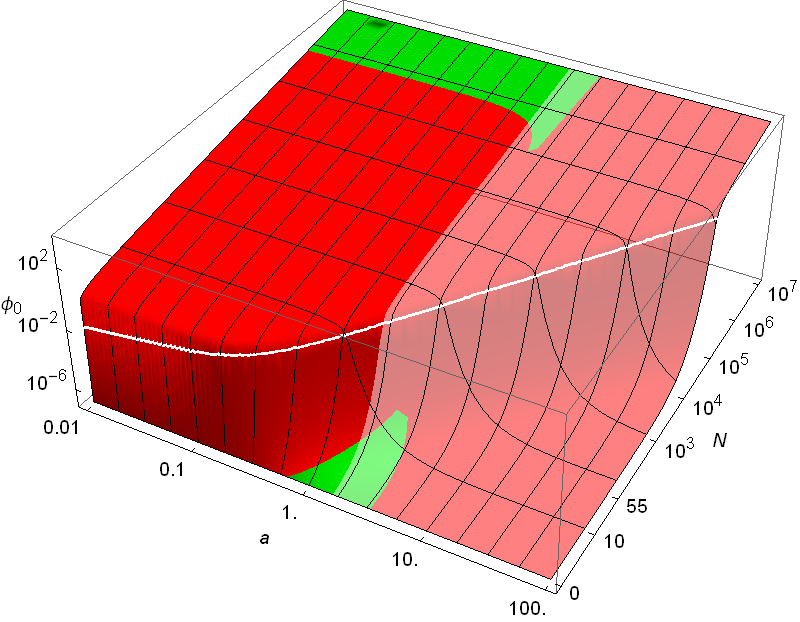
\includegraphics[width=7.5cm]{Figures/phi0_vs_a_N_Eternal_Region}
    \caption{A plot of $\phi(N;\aaa)$, the field value as a function of the number of e-foldings $N$ until the end of inflation and the paramter $\aaa$.  The green shaded regions are those in which stochastic eternal inflation occurs.  The greyed out region is excluded by the constraing on the scalar index $n_s$.  The white line marks the boundary between quadratic and vacuum approximations at $\phi = \aaa$.}
    \label{phi_vs_N_a}
\end{figure}

% \begin{figure}[h]
%     \centering
%     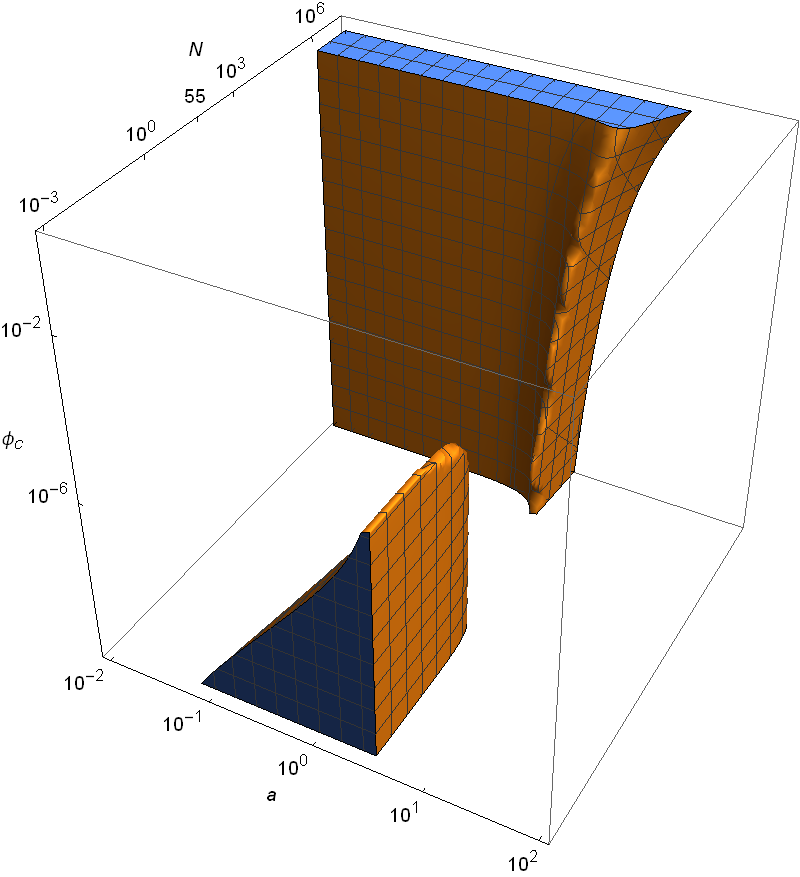
\includegraphics[width=7.5cm]{Figures/RegionPlot_a_N_phi0}
% \end{figure}

\subsubsection{Topological Eternal Inflation}

For $\phi < \phi_c$, the potential has two local minima at $\pm M/\sqrt{\lambda}$.  
In neighboring regions of space that begin with $\sigma$ near its local maximum, the field can roll down the slope in different directions -- toward $-M/\sqrt{\lambda}$ or $+M/\sqrt{\lambda}$.  
This leads to the formation a domain wall in which the field is stuck near the local maximum.  
If the potential near the maximum is sufficiently flat, so that the domain wall thickness exceeds the Hubble radius, then the volume within the wall will inflate faster than it decays, resulting in eternal inflation.
\[ \left. \ddx{^2V}{\sigma^2} \right\rvert_{\sigma=0} \ll \frac{V}{3 M_P^2} \]
\[ g^2 \phi^2 - M^2 \ll \frac{1}{3 M_P^2} \left( \frac{M^4}{4\lambda} + \frac{m^2}{2} \phi^2 \right) \]
\[ \left( g^2 - \frac{4\pi}{3} \, m^2 \right) \phi^2 \ll \left( 1 + \frac{2\pi}{3} \frac{M^2}{\lambda} \right) M^2 \]
If $m \ll 1$ and $M^2 \ll \lambda$, then the potential is sufficiently flat for $\phi \ll \phi_c$.  

We must also assert that the kinetic energy of $\phi$ be sub-dominant -- satisfying the slow roll conditions.  The two can be consistent if the potential is vacuum dominated:
\[ \phi \ll \frac{M^4}{m^2} \frac{M_P}{\lambda} \qquad M^4 \gg \lambda m^2 \]

\[m = 1 \quad m = 10^{-5} \quad m = 10^{-10} \]

\[ \log_{10} \frac{\phi_0}{a} = 0 \quad \log_{10} \frac{\phi_0}{a} = -2 \quad \log_{10} \frac{\phi_0}{a} = 4 \]


    % \[ n_s - 1 = \dfrac{2 m^2}{V} \left( 1 - \dfrac{3 \, m^2 \phi^2}{2 V} \right) M_P^2 = -0.047 \pm 0.016 \]
    % \[ \alpha_s = \dfrac{4 m^4 \phi^2}{V^2} \left( \dfrac{2 m^2}{V} - \dfrac{ 3 m^4 \phi^2}{2 V^2} \right) M_P^4 = -0.040 \pm 0.027 \]



    \section{Numerical Approaches}

\begin{figure*}
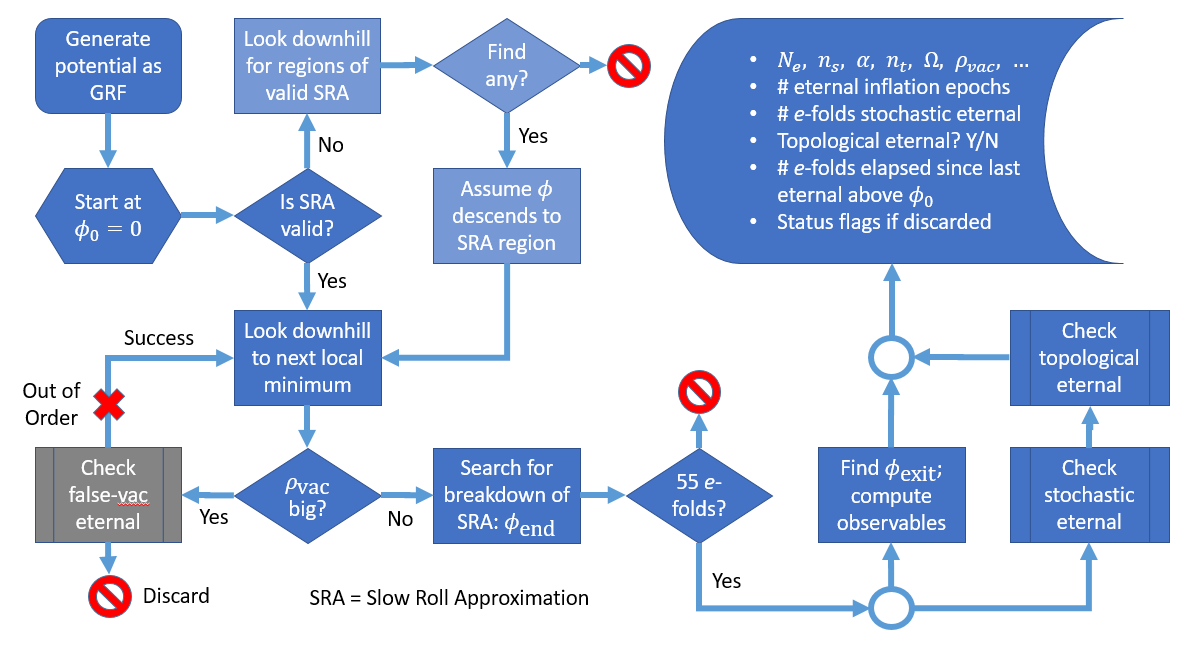
\includegraphics[width=\linewidth]{flowchart}
\end{figure*}

We have reached the limits of applicability of analytical techniques, and now must turn to numerical simulations.

\subsection{Simulating Possible Measures}

% The statement that eternal inflation is or is not generic among a large class of inflation models hides an ambiguity in the choice of measure -– the procedure we adopt for breaking up the space of models for the purpose of assigning probabilities.  The measure establishes the statistical framework in which we assess the likelihood of scenarios like eternal inflation, yet known laws do not appear to single out a preferred measure.  It seems we must make a choice, weighing the merits of possible measures based on factors such as simplicity, alignment with a consistent set of physical principles, and utility in sorting the features that cosmologists are most interested in studying.  

% A measure is a mathematical procedure for assigning a non-negative volume to regions in a space, in such a way that the volume of a subregion is always less than that of its container.  
In the context of inflationary cosmology, we are concerned with measures on the space of viable inflation scenarios -- consisting of a potential function for a single inflaton field and a set of initial conditions (e.g. initial field value).

To explore the consequences of adopting various measures on the space of initial field values, we simulate the dynamics of inflation across an ensemble of randomly generated inflaton potentials.  Following the example of Tegmark, we generate the potential functions as Gaussian random fields.

Since there is always a local maximum to the left and right of any point of the Gaussian random field, there will always be stochastic eternal inflation higher up on the potential slope.

In these simulations, we test for the appearance of stochastic and topological eternal inflation.  Beacuse the Gaussian Random Field has a period much larger than the Planck scale, we could always claim that the field was stuck in a distant false vacuum of the potential before tunneling to the initial value of our simulation.  Searching for false-vacuum eternal inflation would also add enormous costs to the computational complexity of the simulation, since we would need to compute innumerable tunneling amplitudes via an instanton calculation.  We are limiting the simulation to the local half-basin and the half-basins on either side (together a sesqui-basin).  We ignore cases in which inflation ends before the local minimum is reached and the field is able to climb the next hill.

A Gaussian random field (GRF) can be constructed as a superposition of a large number of plane waves, each with the same amplitude and a uniformly distributed random phase.  Following the central limit theorem, the distribution of the field value at any point will approach Gaussian as the number of such plane wave contributions becomes large.  If the potential governing the inflaton owes its form to an interaction with another quantum field.  The Gaussian random potential is (1) bounded from above and below, with arbitrarily large peaks occuring arbitrarily infrequently; (2) contiuous and smooth; and (3) .

We express the potential $V(\phi) = m_v^4 f(\phi/m_h)$ in terms of a dimensionless Gaussian random field
\[ f(x) = \frac{a_0}{2} + \sum_k a_k \cos(kx) + \sum_k a_{-k} \sin(kx) \]
and constants defining the mass scales of the potential ($m_v$) and the field ($m_h$).
The coefficients $a_k$ are sampled from a Gaussian distribution such that 
\[ \text{Var} (a_k) = q^\gamma e^{-q^2/2}, \qquad q \equiv {k}/{k_{\text{max}}} \]

\paragraph{Measure A} The simulation sets the initial field value at $\phi = 0$.

\paragraph{Measure B} Start at the nearest local maximum with $\dot\phi = 0$.

We must enforce constraints so that the observed features of the cosmic microwave background are reproduced by these models.

\begin{enumerate}

\item
Initialize the field according to one of the measures listed above.

\item
Check for topological eternal inflation.  If quantum fluctuations with width $\delta\phi = H/2\pi$ could take the field from its initial value to the nearest local maximum of the potential with probability greater than $ 1/e^3$, evaluate the criterion for topological eternal inflation at that maximum.

\item
Check for stochastic eternal inflation at the maximum.  If the slow roll conditions break down within a Hubble time of classical evolution, then consider approximations invalid -- no stochastic eternal inflation at the maximum.

\item
If the criteria for slow roll inflation are met at the starting point, search the future of the field's classical downhill trajectory for a breakdown of the slow roll conditions.

\item
Evaluate the stochastic eternal inflation criterion \eqref{seic} for field values between the nearest local maximum (past) and the end of slow roll inflation (future).  Record the number of e-foldings that elapse between the breakdown of the SEIC and the end of inflation.

\item
If the field gets trapped in a local minimum, assume that the quantum tunneling rate is sufficiently high, and evaluate the likelihood of false-vacuum eternal inflation.

\end{enumerate}

\begin{figure}
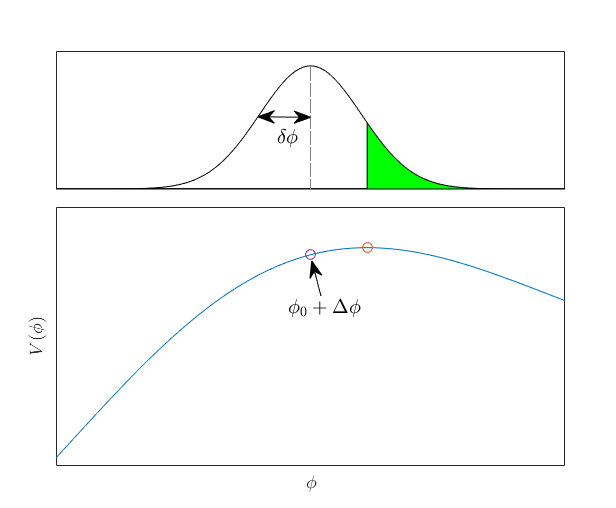
\includegraphics[width=8cm]{topologicalPlot}
\caption{Topological criterion}
\end{figure}
% \[ \sigma_{V^{(k)}(\phi)}^2 = \left( \prod_{i=1}^k \frac{2k-1}{m_h} \right) \sigma_{V(\phi)}^2 \]

\begin{figure}
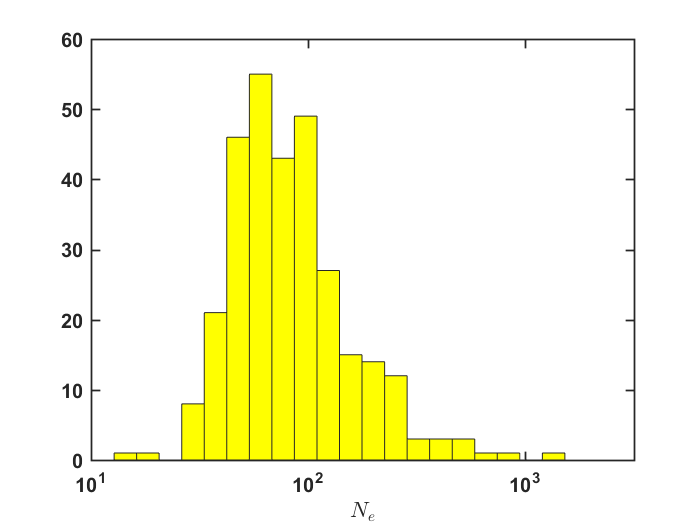
\includegraphics[width=8cm]{NsinceEternal}
\caption{Number of e-foldings elapsed between the breakdown of the stochastic eternal inflation criterion and the starting point. ($m_v = 0.007,\; m_h = 5$)  No constraints were imposed on other parameters.}
\end{figure}

Effects of shifting the potential by $-\rho_\Lambda$:
\begin{align*}
\delta N &= -\int \frac{\rho_\Lambda}{V'} \,\dx \phi \\
\delta Q &= + \mathcal O(\delta \rho_\Lambda^2) \\
\delta r &= 2 r \frac{\rho_\Lambda}{\rho_{\text{exit}}} + \mathcal O(\delta \rho_\Lambda^2) \\
\delta n_s &= \left((n_s - 1) - 6 \epsilon \right) \frac{\rho_\Lambda}{\rho_{\text{exit}}} + \mathcal O(\rho_\Lambda^2) \\
\delta \alpha &= + \mathcal O(\delta \rho_\Lambda^2) \\
\delta n_t &= 2 n_t \frac{\rho_\Lambda}{\rho_{\text{exit}}} + \mathcal O(\delta \rho_\Lambda^2) \\
\delta(\ln \Omega_k) &= + \mathcal O(\delta \rho_\Lambda^2) \\
\delta(\ln \rho) &= + \mathcal O(\delta \rho_\Lambda^2) 
\end{align*}

% \subsection{Genetic Algorithm}

% \begin{enumerate}

% \item
% Randomly generate a population of half-basins of the inflaton potential $V(\phi)$.  These can be generated by first generating a Gaussian random field, and then breaking it up into half-basins.

% \item
% Compute the value of a fitness function for each half-basin, which rewards or penalizes particular characteristics of the potential segment.  For example, the fitness function could maximize the number of e-foldings of inflation.

% \item
% Sort members of the population by fitness.  Breed high performers with other high performers, and discard the worst performers.

% \item
% Check criteria for success at each generation.  Run many iterations of the genetic algorithm, and record the convergence time in each case.  Compare convergence times among different fitness functions to get a relative measure of the genericness of different outcomes.

% \end{enumerate}

We collected the following parameters from each run of the simulation:
\begin{itemize}
\item Number of eternal inflation epochs
\item Duration of each epoch (in e-foldings)
\item If eternal inflation occurred higher up on the potential than the starting point, how many e-foldings of inflation elapsed between the end of the most recent epoch and the starting point.
\item 
\end{itemize}
\paragraph{Next Steps}

\begin{itemize}
\item Enforce constraints on parameters (e.g. $Q_s$, $n_s$) when generating potentials.
\item Express observables ($n_s$, $\alpha_s$, $Q_s$, etc.) in terms of the potential and its derivatives ($V(\phi)$, $V'(\phi)$, etc.).  Compute probability distributions for the potential and its derivatives, and in turn for observables.
\[ n_s = 1 - 6\epsilon + 2\eta = 1 - 3 \left( \frac{V'}{V} \right)^2 + 2 \frac{V''}{V} \]
\[ \alpha = 16\epsilon\eta - 24 \epsilon^2 - 2 \xi_2 \]
\end{itemize}

% \subsection{Designer Inflation Models}

% \paragraph{Genetic Algorithm}

% \paragraph{Optimization}
    \section{Discussion and Conclusions}

Evidence for some kind of past inflationary epoch is mounting, although empirical tests have yet to pick out a single, preferred model of inflation from the vast space of candidate models.  So if eternal inflation really were a nearly inevitable implication of any simple inflation mechanism, we would be forced to take very seriously the multiverse conjecture and confront the thorny questions it presents.  Chief among these is the measure problem: how are we to interpret probabilities and make sensible predictions in cosmology if every possible configuration of any subsystem is in principle realized an infinite number of times?

Questions
\begin{itemize}

\item If we assume that the inflaton is a quantum field, will terms in the potential containing odd multiples of the field operator contribute?  Is the state $\Psi$ in which we evaluate $\expv{\phi} = \bra{\Psi}\hat\phi\ket{\Psi}$ one with a definite number of particles?

\item Should we allow the potential to go negative?

\end{itemize}

\subsection{Future Work}

It would be of interest to generalize the numerical methods presented in this work to include multifield models, in which the dynamics are potentially much more complicated.

So why don't we go

somewhere only $W^{\pm}$
    
    \appendix
    \section{Instantons}

% \[ H^2 ds^2 = -\dx t^2 + \sin^2(r) \left( \dx \xi^2 + \cosh^2 \xi \left( \dx \tilde\theta^2 + \sinh^2 \tilde\theta \, \dx\phi^2 \right) \right) \]
% \[ r \equiv it \qquad \rho \equiv H^{-1} \sin(r) \]
% \[ ds^2 = H^{-2} \dx r^2 + \rho(r)^2 \left( \dx \xi^2 + \cosh^2 \xi \left( \dx \tilde\theta^2 + \sinh^2 \tilde\theta \, \dx\phi^2 \right) \right) \]
The equations of motion for the field $\phi$ and the Euclidean radial coordinate $\rho$ are
\[ \phi'' + \frac{3 \rho'}{\rho} \phi' = \ddx{V}{\phi} \qquad \rho'' = -\frac{8\pi}{3M_{Pl}^2} \left( \phi'^2 + V(\phi) \right) \]
% The radial component of Einstein's field equations is
% \[ \ddot\rho = -\frac{8\pi}{3M_{Pl}^2} \left( \dot\phi^2 + V(\phi) \right) \]
The tunneling amplitude for a single instanton in terms of the Euclidean action $S_E$ is given by
The probability amplitude for the field at a point to transition from the false vacuum to the true vacuum in a time $\tau = t_f - t_0$ along the path $\bar\phi(t)$ is
\[ K = \bra{\phi_T,t_f} \left[ \overset\leftarrow\prod_i \ket{\bar\phi_i,t_i}\bra{\bar\phi_i,t_i} \hat U(t_{i-1},t_i) \right] \ket{\phi_F,t_0} = \exp(-S_E) \]
% \[ K = \exp \left( - S_E / \hbar \right) \]
\[ S_E(\xi,r,\theta,\phi) = \int \dx\tau \,\dx^3 x \,\sqrt{g} \, \left[ \frac12 \dot\phi^2 + V(\phi) + \frac{1}{2\kappa} \tilde R(\rho) \right] \]
Here the overdot denotes a total derivative with respect to Euclidean time $\tau = -it$.  The histories that have the most weight will be those that minimize the Euclidean action.  Taking into account those paths that can be course-grained as corresponding to the instanton path, we have
\[ K = \int D\delta\phi \, \exp(-S_E[\bar\phi+\delta\phi,\bar\rho]) \]
For now, we fix the background geometry to that of the instanton solution.  The highest degree of constructive interference occurs near the classical and semi-classical solutions -- those that extremize the action and the Euclidean action.  We are therefore concerned with functions that differ from those solutions by only a small perturbation.  Expanding the Euclidean action around the instanton solution, we obtain
\[ S_E[\phi,\rho] \approx S_E[\bar\phi,\bar\rho] + \frac12 \int \dx\xi_1 \dx\xi_2 \left. \fdx{^2S_E}{\phi(\xi_1) \delta\phi(\xi_2)} \right\rvert_{\bar\phi} \delta\phi(\xi_1) \delta\phi(\xi_2) \]
Recasting the integral as a quadratic form, we have
\[ S_E[\phi,\rho] \approx S_E[\bar\phi,\bar\rho] + \frac12 {\mathbf \Phi}^{\mathrm T} \mathbf\Sigma^{-1} \mathbf\Phi \]
with \[ \Sigma^{-1} \equiv \fdx{^2 S_E[\phi,\bar\rho]}{\phi(\xi_1) \delta\phi(\xi_2)} = 2 \pi \rho^3 \delta(\xi_1-\xi_2) \, \left. \pdx{^2V}{\phi^2} \right\rvert_{\bar\phi(\xi_1)} \]
The integral over paths then becomes a Gaussian integral, with $\mathbf\Sigma$ the covariance matrix.
\begin{align*}
 A &= \int \mathrm D \Phi \, \exp \left( -\frac12 \mathbf\Phi^{\mathrm T} \mathbf\Sigma^{-1} \mathbf\Phi \right) = \left[ \det \left( \frac{ \mathbf\Sigma^{-1} }{2\pi} \right) \right]^{-1/2} \\
 A &= \left[ \prod_i \left( \left. \frac{2\pi^2 \rho(\xi_i)^3}{2\pi} \pdx{^2V}{\phi^2} \right\rvert_{\phi(\xi_i)} \right)  \right]^{-1/2} \\
 A &= \exp \left[ -\frac12 \int \dx\xi \, \log \left( \left. \pi \rho(\xi)^3 \pdx{^2V}{\phi^2} \right\rvert_{\bar\phi(\xi)} \right)  \right]
\end{align*}
 \[ \int_{-\Lambda}^{\Lambda} \dx x \, \exp \left( -\frac{x^2}{2a^2} \right) = \sqrt{2\pi} a \, \mathrm{erf} \left( \frac{\Lambda}{a\sqrt{2}} \right) \approx 2\Lambda \left[ 1 - \frac16 \frac{\Lambda^2}{a^2} \right] \]
 For a diagonal covariance matrix $\mathbf \Sigma$ and expanded in the small parameter $\Lambda$, the integral is
 \[ \int_{-\Lambda}^{\Lambda} Dx \, \exp \left( -\frac12 \mathbf x^{\mathrm T} \mathbf \Sigma^{-1} \mathbf x \right) \approx (2 \Lambda)^{d} \left[ \sum_{i=1}^d \left( 1 - \frac16 \frac{\Lambda^2}{\sigma_i^2} \right) \right] \]

% \[ \dx s^2 = \dx r^2 + \rho(r)^2 \dx\Omega^2 \]
% The coordinates $r$ and $\Omega$ correspond to the radius of and solid angle on a 3-sphere.
% \[ S_E = \int \dx r \, L \!\left[\phi(r),\dot\phi(r),\rho(r),\dot\rho(r),\ddot\rho(r)\right] = 2 \pi^2 \int \dx r \left[ \rho^3 \left( \frac12 \dot\phi^2 + V(\phi) \right) + \frac{3}{\kappa} \left( \rho^2 \ddot\rho + \rho \dot\rho^2 - \rho \right) \right] \]
% Note that the first functional derivatives of $S_E$ vanish when evaluated for the instanton solution.
% \[ \fdx{S_E}{\phi(r_1)} = \pdx{S}{\phi(r_1)} - \ddx{}{r} \pdx{S}{\dot\phi(r_1)} \]
% \[ \fdx{^2S_E}{\phi(r_1)\delta\phi(r_2)} = \left. \left( \pdx{^2\mathcal L}{\phi^2} + \frac12 \ddx{}{\xi^2} \pdx{}{\ddot\phi} \left[ \ddx{}{\xi} \pdx{\mathcal L}{\dot\phi} \right] \right) \right\rvert_{r_1} \delta(r_1-r_2) \]
% \[ \fdx{^2S_E}{\phi(r_1)\delta\phi(r_2)} = 2 \pi^2 \rho^3 \left. \pdx{^2V}{\phi^2} \right\rvert_{r_1} \delta(r_1-r_2) \]
% \[ \fdx{S_E}{\phi} = \pdx{S}{\rho} - \ddx{}{\xi} \pdx{S}{\dot\rho} + \frac12 \ddx{}{\xi^2} \pdx{^2S}{\ddot\rho} \]

The amplitude is then
\[ K = A \exp \left(-S_E \left[\bar\phi,\bar\rho \right] \right) = \exp \left[ - \left(S_E + \frac12 \int \dx \xi \, \ln \left(\pi\rho(\xi)^3 \left. \ddx{^2V}{\phi^2} \right\rvert_{\bar\phi(\xi)} \right) \right) \right] \]


The probability per unit volume that a bubble has {\it not} formed -- that at time $t_f$, the field configuration contains no true vacuum -- is
\[ K = \sum_{\phi_f \neq \phi_F} \bra{\phi_f,t_f} \left[ \overset\leftarrow\prod_i \ket{\bar\phi_i,t_i}\bra{\bar\phi_i,t_i} \hat U(t_{i-1},t_i) \right] \ket{\phi_F,t_0} \abs{K}^2 \]
Among the paths that do not lead to the appearance of regions of true vacuum, the dominant contribution is the classical solution , which extremizes the classical action $S$.  (The next leading contributions come from consecutive of instanton-anti-instanton transitions.)
\[ K \approx K_{cl} = \exp(-i S_{cl}) \] 
The corresponding probability is
\[ P = \abs{K}^2 \equiv \exp(-\Gamma (t_f - t_0) ) \]
\[ \Gamma = \lim_{t_0 \to \infty} (- \ddx{}{t} \ln P) \]
\[ K = \sum_{\bar\phi} \bra{\phi_T,t_f} \left[ \overset\leftarrow\prod_i \ket{\bar\phi_i,t_i}\bra{\bar\phi_i,t_i} \hat U(t_{i-1},t_i) \right] \ket{\phi_F,t_0} = \exp(-S_E[\bar\phi(x,t)]) \]

In computing the tunneling amplitude with endpoints matching those of the instanton solution, we have as the pre-factor an approximately Gaussian integral evaluated over the neighborhood of the instanton solution.
\[ \exp \left(-\Gamma (t_1 - t_0) \right) = \frac{\bra{\Omega} \hat U(t_0,t_1) \ket{0} \! \bra{0} \hat U(t_0,t_1) \ket{\Omega}}{\braket{\Omega}{\Omega}} = \frac{\bra{\Omega} \hat O \ket{\Omega}}{\braket{\Omega}{\Omega}} \]
\[ \hat O \equiv \hat U(\tau) \ket{0} \! \bra{0} \hat U(\tau) \]
\[ \exp \left(-\Gamma (t_1 - t_0) \right) = \frac{\bra{\Omega} \hat U(t_0,t_1) \ket{0} \! \bra{0} \hat U(t_0,t_1) \ket{\Omega}}{\braket{\Omega}{\Omega}} = \frac{\bra{\Omega} \hat O \ket{\Omega}}{\braket{\Omega}{\Omega}} \]
\[ K = \bra{\Omega_1} U(t_0,t_1) \ket{\Omega_0} = A \exp(-S_E[\bar\phi,\bar\rho]) \]
\[ A \approx \int D\delta\phi \, \exp \left(- \pi^2 \int \dx\xi \, \rho(\xi)^3 \left. \ddx{^2V}{\phi^2} \right\rvert_{\bar\phi} \delta\phi(\xi)^2 \right) \]
\[ A \approx \int \delta\phi_1 \int \delta\phi_2 \cdots \int \delta\phi_N \, \exp \left(- \sum_{i=1}^N \pi^2 \rho_i^3 \left. \ddx{^2V}{\phi^2} \right\rvert_{\bar\phi_i} \delta\phi_i^2 \right) \]

We consider the case of a single instanton, as well as those of multiple widely separated in time, as resulting in a false vacuum tunneling event.
\[ \frac{\Lambda}{V} = \left[ \frac{K_1 + K_2 + K_3 + \cdots}{K_0 + K_1 + K_2 + \cdots} \right]^2 \approx \left[ \frac{K_1}{K_0 + K_1} \right]^2 \]

In flat space
\[ \frac{\Gamma}{V} = \left( \frac{\mathcal M S_3(R_0)}{8\pi} \right)^2 \fract{4 R_0^{-4}}{\pi^2} e^{\zeta'_{R}(-2)} e^{-\bar S_E} \overset?= \lambda \]
In de Sitter space
\[ \ddx{\mathcal N}{V_{phys}} \approx \frac{\abs{\lambda}}{H^d} \frac{\dx R}{R^d} \]
    
    % \bibliographystyle{unsrt}
    % \bibliography{reference}
    \printbibliography
    
\end{document}

